%% %%%%%%%%%%%%%%%%%%%%%%%%%%%%%%%%%%%%%%%%%%%%%%%%
%% Problem Set/Assignment Template to be used by the
%% Food and Resource Economics Department - IFAS
%% University of Florida's graduates.
%% %%%%%%%%%%%%%%%%%%%%%%%%%%%%%%%%%%%%%%%%%%%%%%%%
%% Version 1.0 - November 2019
%% %%%%%%%%%%%%%%%%%%%%%%%%%%%%%%%%%%%%%%%%%%%%%%%%
%% Ariel Soto-Caro
%%  - asotocaro@ufl.edu
%%  - arielsotocaro@gmail.com
%% %%%%%%%%%%%%%%%%%%%%%%%%%%%%%%%%%%%%%%%%%%%%%%%%

\documentclass[12pt]{article}
\usepackage{design_ASC}

\setlength\parindent{0pt} %% Do not touch this

%% -----------------------------
%% TITLE
%% -----------------------------
\title{IDbyDNA code challange} %% Title

\author{Hanie Samimi}%% Author's name

\date{\today} %% Change "\today" by another date manually
%% -----------------------------
%% -----------------------------

%% %%%%%%%%%%%%%%%%%%%%%%%%%
\begin{document}
\setlength{\droptitle}{-5em}    
%% %%%%%%%%%%%%%%%%%%%%%%%%%
\maketitle

% --------------------------
% Start here
% --------------------------

% %%%%%%%%%%%%%%%%%%%
\section*{Question 3}
% %%%%%%%%%%%%%%%%%%%
{\bfseries In your own words, write a brief technical methods section describing Sensitivity and Specificity as related to scoring the performance of a diagnostic test}

(LaTex is preferred)
% %%%%%%%%%%%%%%%%%%%
\subsection*{Answer}
% %%%%%%%%%%%%%%%%%%%
Diagnostic tests have different meanings in different fields. In general, a diagnostic test is
a tool to answer to a yes or no question about a sample's condition. The answer should be determined based on sample's features and conditions. For example, BMI is a tool which determines if a person is overweight or not. The BMI uses the height and current weight of each person and computes it's .... based on that, it measures the .... and determines if the person is overweight.
Since any diagnostic tests guess the answer based on samples features, there could be a possibility that the answer is wrong. For instance, laboratory tests such as surgery, can determine the presence of any symptom in liver with highest accuracy. However, these methods have side effects,too.\\
An alternative solution could be using X-ray scan of the liver. To find the accuracy of the results of X-ray, we can use a confusion matrix. A confusion matrix is table that visualize the classification of samples based on their actual conditional and predicted condition using a diagnosis test. Below is a sample of confusion matrix for a group of 344 patients. Each row shows the classification based on X-ray scan while columns shows it based on laboratory tests.   

\begin{figure}
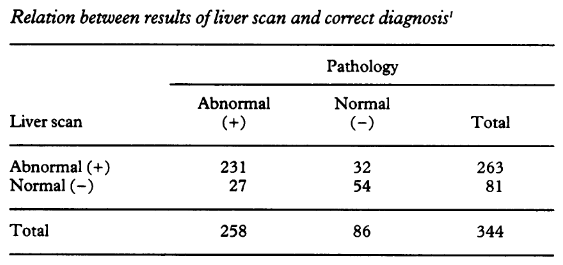
\includegraphics[width=\textwidth]{confusionMatrix.png}
\caption{Confusion matrix for liver cancer test. Rows show the classification based on X-ray test while columns are results based on laboratory test.} \label{fig1}
\end{figure}

The table shows that there are 231 cases that are predicted with liver abnormal condition based on both X-ray and laboratory test. However, there are 27 cases that had abnormality based on the laboratory test while X-ray test failed to identify. On the other hand, there are 54 cases that have normal liver condition based on both X-ray and laboratory test. In addition, 32 cases were symptom free while X-ray test labeled them as Abnormal. 
These numbers show us the number of times that the X-ray was as accurate as liver scan test. To score the accuracy of X-ray test and compare it alternative ones, we need to compute four values using the confusion matrix: 
\begin{itemize}
\item True positive: Number of Abnormal cases based on both tests 
\item True negative: Number of Normal cases based on both test test
\item False positive: Number of Normal cases that are predicted as Abnormal by x-ray test 
\item False negative: Number of Abnormal cases that are predicted as normal by x-ray test
\end{itemize}
Figure shows these four numbers for 231 cases of the study. These numbers are being used to compute two scores called Sensitivity and Specificity. These scores were first defined  Jacob Yerushalmy, an American bio-statistician in 1947. Sensitivity or true-positive rate shows the ratio of Abnormal cases that are diagnosed with symptom among to all cases that have been diagnosed with symptom. Specificity or true-negative rate is the ratio of normal cases that are diagnosed symptom free to all normal cases.\\
In reality, there is a trade-off between increasing these two scores.Higher values of sensitivity shows that results for cases that are diagnosed with symptoms are reliable. Higher specificity shows that the chance that the chance of mislabeling Normal case with an Abnormal label is very low. To increase sensitivity, the tool will label cases with week symptoms as abnormal. It will increase the chance of finding more abnormal case while increase the chance of mislabeling and decrease specificity. On the other hand, labeling normal to cases with week symptoms decreases the chance of finding abnormal cases and results in lower sensitivity.
While these scores are important to select a test, they can not gaurantee that tests results will be highly reliable for all situations. 

In conclusion, the interpretation of the two scores, specificity and sensitivity depends on the population that is being tested. While higher scores shows a better detecting performance, it does not guarantee highest accuracy in all situations. 






\end{document}